\chapter{Principles of Nuclear Magnetic Resonance Imaging}
\label{chap:Theory}
\newpage
\begin{abstract}
	This chapter outlines the theoretical framework behind \ac*{NMR} and \ac*{MRI}. Beginning with an overview of nuclear spin and resonance, the origin of the signal measured in \ac{NMR} is explained. The processes responsible for variations within signals such as relaxation mechanisms are then outlined and the techniques used to measure these different signals described. Finally, an overview of the process by which the signals can be used to form images is given, covering concepts such as spacial localisation, image acquisition schemes and acceleration methods.
	%\lipsum[1]
\end{abstract}
\newpage

\section{Source of the NMR Signal}
\label{sec:theory_source_of_nmr}

\subsection{Nuclear Spin}
\label{subsec:theory_nuclear_spin}
The \ac{NMR} signal arises from the interaction between the atomic nucleus and an external magnetic field. These atomic nuclei possess intrinsic properties of, mass ($m$), charge ($q$) and spin ($I$). Spin is a quantum mechanical property and as such, can only take values of half integers or integers. Nuclear spin is dictated by the sum of the constituent particles of the nucleus, protons and neutrons, each of which posses their own spin of either $\sfrac{1}{2}$ or $-\sfrac{1}{2}$ respectively. The additive nature of nuclear spin means that pairs of nucleons can cancel out leaving the nucleus with zero net spin, this happens when the nuclei contains an even number of protons and neutrons. If the nuclei contains an odd number of both protons and neutrons, it will have a positive integer nuclear spin whereas if the nuclei has an odd number of protons or neutrons, it will have a half integer spin. 

%\subsection{Nuclear Magnetisation}

The spin angular momentum, $\mathbf{J}$ of a nucleus of spin $I$ is given by
\begin{equation}
\left|\mathbf{J}\right| = \hbar \sqrt{I\left(I+1\right)}
\label{eq:theory_angular_momentum}
\end{equation}
where $\hbar$ is the reduced Plank's constant, $\sfrac{h}{2\pi}$. As the nucleus is charged and rotating, it gives rise to a current and therefore a magnetic moment $\bm{\mu}$,
\begin{equation}
\bm{\mu}=\gamma \mathbf{J}
\label{eq:theory_magnetic_moment}
\end{equation}
where $\gamma$ is the gyromagnetic ration for the nucleus, a constant which depends on the charge and mass of the nucleus. Table \ref{tab:theory_isotope_spin_gmr} shows the gyromagnetic ratio ($\gamma$) and nuclear spin ($I$) of common \ac{NMR} sensitive isotopes \cite{harris_nmr_1976, bernstein_handbook_2004, westbrook_mri_2015}. Due to its high gyromagnetic ratio, compared to other nuclei used for \ac{NMR}, and relative abundance in the body, \ce{^{1}H}, a single proton, is most commonly used for \ac{MRI}.

\begin{table}[H]
	\centering
	\begin{tabular}{lccc}
		\hline
		Isotope            & Spin & $\gamma$ (MHzT$^{-1}$)                     & Sensitivity Relative to \ce{^{1}H}     \\ \hline
		\ce{^{1}H}         & $\sfrac{1}{2}$  & 42.58                                      & 1                                      \\
		\ce{^{2}H}         & $1$    & 6.54                                       & 0.0097                                 \\
		\ce{^{13}C}        & $\sfrac{1}{2}$  & 10.71                                      & 0.016                                  \\
		\ce{^{19}F}        & $\sfrac{1}{2}$  & 40.05                                      & 0.83                                   \\
		\ce{^{23}Na}       & $\sfrac{3}{2}$  & 11.27                                      & 0.093                                  \\
		\ce{^{31}P}        & $\sfrac{1}{2}$  & 17.25                                      & 0.066                                  \\ \hline
	\end{tabular}
	\caption{Common \ac{NMR} isotopes, their nuclear spin, gyromagnetic ratio and sensitivity, relative to \ce{^{1}H}.}
	\label{tab:theory_isotope_spin_gmr}
\end{table}

\subsection{Application of an External Magnetic Field}
If we consider the hydrogen nuclei in a sample of tissue, the number of possible eigenstates for a nuclear spin $I$ is $\left(2I + 1\right)$. This means that for the \ce{^{1}H} nuclei in our sample, where $I=\sfrac{1}{2}$, we can observe two possible eigenstates, $\left| + \sfrac{1}{2} \right \rangle$ and $\left| - \sfrac{1}{2} \right \rangle$ often written as $\left|  \uparrow \right \rangle$ and $\left|  \downarrow \right \rangle$. In the absence of an external magnetic field, these states are degenerate as they have the same energy, however, if we move our sample into a static external magnetic field along the $z$-axis, $B_0$, the energy levels separate.

The $z$-component of the magnetic moment is defined by,
\begin{equation}
\mu_z=\gamma \hbar m_I
\label{eq:theory_longitudinal_magnetic_moment}
\end{equation}
where $m_I$ are the possible spin quantum numbers of the nucleus. For our proton system with spin $\sfrac{1}{2}$, $\mu_z$ is given by
\begin{equation}
\mu_z = \pm \frac{1}{2}\gamma\hbar.
\end{equation}
The spins can either be aligned parallel to the external magnetic field in the lower energy of the two eigenstates, also known as spin up; or anti-parallel to the magnetic field in the higher energy eigenstate, spin down. The energy difference between these two eigenstates is given by,
\begin{equation}
\Delta E = \gamma \hbar B_0.
\label{eq:theory_zeeman}
\end{equation}

For an ensemble of spins in an external magnetic field, there will be an imbalance between the populations of each state, with more spins occupying the lower of the two energy states. The net magnetisation of the sample is simply the sum of the constituent spins and as such, the application of an external magnetic field leads to the sample gaining a net magnetisation vector, $\mathbf{M}$, aligned with $B_0$. This effect is very small, the magnitude of the imbalance between eigenstates can be derived from Boltzmann statistics and is given by,
\begin{equation}
\frac{N_{\uparrow}}{N_{\downarrow}} = \exp \left(\frac{\Delta E}{k_B T}\right),
\label{eq:theory_boltzman}
\end{equation}
where $N_{\downarrow}$ and $N_{\uparrow}$ are the the number of spins aligned with and against $B_0$ respectively, $k_B$ is Boltzmann's constant and $T$ is the temperature of the system. This means that for a sample of biological tissue at body temperature in a 3T magnetic field, the population difference is very small at approximately three parts per million. Although this measurable proportion is very small, it can be detected due to the high density of protons in the tissue. The signal can be increased by the application of a stronger main magnetic field, $B_0$, Figure \ref{fig:theory_precession}.

\begin{figure}[H]
	\centering
	\begin{subfigure}[c]{0.47\textwidth}
		\centering
		\includegraphics[width=1\textwidth]{Theory/precession/precession_equilibrium.eps}
		\caption{No external magnetic field}
		\label{fig:theory_precession_eq}
	\end{subfigure}
	\hfill
	\begin{subfigure}[c]{0.47\textwidth}
		\centering
		\includegraphics[width=1\textwidth]{Theory/precession/precession_b0.eps}
		\caption{External magnetic field, $B_0$, applied}
		\label{fig:theory_precession_b0}
	\end{subfigure}
	\caption{Initially the magnetic moments are randomly distributed (\subref{fig:theory_precession_eq}). Upon the application of the external magnetic field, $B_0$, the magnetic moments align either parallel or anti-parallel to the external field and precess at the Larmor frequency, $\omega_0$ (\subref{fig:theory_precession_b0}).}
	\label{fig:theory_precession}
\end{figure}

\subsection{Precession}
%The nuclear magnetic moment always has a transverse component as from equations \eqref{eq:theory_angular_momentum}, \eqref{eq:theory_magnetic_moment} and \eqref{eq:theory_longitudinal_magnetic_moment} we can see $\left| \bm{\mu} \right| > \mu_z$, and therefore the magnetic moment cannot exactly align along the $z$-axis. This misalignment between $\bm{\mu}$ and $B_0$ causes $\bm{\mu}$ to precess around $B_0$ at an angular frequency $\omega_0$, known as the Larmor frequency and is given by,
%\begin{equation}
%\omega_0=\gamma B_0.
%\end{equation}

Classically, if a magnetic moment, $\bm{\mu}$, is placed into an external magnetic field, $\mathbf{B}$, it will experience a torque, $\tau$, proportional to the change in angular momentum and thus induce a rotation.
\begin{equation}
\bm{\mu} \times \mathbf{B} = \frac{d\mathbf{J}}{dt} = \tau
\label{eq:theory_classical_torque}
\end{equation}
From \eqref{eq:theory_magnetic_moment} the quantum equivalent of \eqref{eq:theory_classical_torque} is the standard form of the Bloch equation \cite{bloch_nuclear_1946},
\begin{equation}
\frac{d\bm{\mu}}{dt} = \gamma \bm{\mu} \times \mathbf{B}
\label{eq:theory_bloch_standard}
\end{equation}
This equation states that if the magnetic moment, $\bm{\mu}$ is not aligned with the external magnetic field, $\mathbf{B}$, it will precess about $\mathbf{B}$. The frequency of this precession, $\omega_0$, is known as the Larmor frequency and is given by substituting Bohr's frequency condition of the Planck relation ($\Delta E = \hbar \omega $) into \eqref{eq:theory_zeeman},
\begin{equation}
\omega_0=\gamma B_0,
\label{eq:theory_larmor}
\end{equation}
Nuclei with a positive gyromagnetic ratio precess clockwise, whereas nuclei (and the electron) with a negative gyromagnetic ratio precess anti-clockwise. For a proton in a 3T magnetic field, the Larmor frequency is 128 MHz.

\subsection{Resonance}

Resonance is the process of energy transfer into a system by the application of energy at the natural frequency of the system. In the case of \ac{NMR} this is the application of an \ac{RF} pulse, also known as $B_1$ field, near the Larmor frequency. Before the \ac{RF} pulse is applied, the spins are at equilibrium, aligned with $B_0$. Upon application of a $B_1$ field close to the Larmor frequency of the target nucleus and perpendicular to $B_0$, the spins aligned with $B_0$ will be displaced from equilibrium and thus precession is induced. The longer the $B_1$ field is applied, the more the net magnetisation vector is displaced, or tipped, away from $B_0$, this allows arbitrary flip angles, $\alpha$, to be achieved, \eqref{eq:theory_flip_angle}. 
\begin{equation}
\alpha = \int_{0}^{T} \gamma B_1\left(t\right) dt
\label{eq:theory_flip_angle}
\end{equation}
In addition to displacing the spins, the $B_1$ field also induces phase coherence within the ensemble making up the net magnetisation vector. When considering the effects of \ac{RF} pulses, it can often be simpler to imagine the system from a reference frame rotating about the $z$-axis at the Larmor frequency. This has the effect of making $B_1$ stationary along the $x$-axis. Figure \ref{fig:theory_reference_frames} shows the evolution of a spin in both the laboratory and rotating frame after the application of a 90$\degree$  \ac{RF} pulse. In both figures the spin is tipped into the transverse plane, $M_{xy}$.

\begin{figure}[H]
	\centering
	\begin{subfigure}[c]{0.47\textwidth}
		\centering
		\includegraphics[width=1\textwidth]{Theory/Rotating_Frame/lab_frame.eps}
		\caption{Laboratory Frame}
		\label{fig:thoery_lab_frame}
	\end{subfigure}
	\hfill
	\begin{subfigure}[c]{0.47\textwidth}
		\centering
		\includegraphics[width=1\textwidth]{Theory/Rotating_Frame/rotating_frame.eps}
		\caption{Rotating Frame}
		\label{fig:theory_rotating_frame}
	\end{subfigure}
	\caption{The laboratory frame of reference shows the procession of the spin about $B_0$ while in the rotating frame, the spin simply rotates about the $x'$-axis}
	\label{fig:theory_reference_frames}
\end{figure}

\section{Relaxation and Contrast Mechanisms}
If disturbed from equilibrium by an \ac{RF} pulse, the net magnetisation vector will not remain in this new state ad infinitum, instead, once the \ac{RF} pulse has been turned off the magnetisation will transition back to its equilibrium state in a process known as relaxation. The time constants characterising the relaxation process vary depending on the environment the spins are in and as such, can vary between different biological tissues. These relaxation constants are the principle source of contrast in \ac{MRI}. Mathematically, this relaxation is described by the full form of the Bloch equation, \eqref{eq:theory_bloch_full},

\begin{equation}
\frac{d\mathbf{M}}{dt} = \gamma \left( \mathbf{M \times B} \right) - \frac{\left( M_z - M_0 \right)}{T_1}\mathbf{\hat{z}} - \frac{M_x \mathbf{\hat{x}} + M_y \mathbf{\hat{y}}}{T_2},
\label{eq:theory_bloch_full}
\end{equation}
where \tone is the longitudinal relaxation time and \ttwo the transverse relaxation time.

\subsection{Longitudinal Relaxation (\tone)}
\label{subsec:theory_t1}
Upon excitation, energy is exchanged between the spin system and the surrounding environment. The result of this energy exchange is that the energy of the spin system decreases and the longitudinal magnetisation exponentially decays to its equilibrium position. The time constant of this exponential decay returning to equilibrium, $M_0$, is known as the longitudinal relaxation time or \tone and is dictated by the efficiency of energy transfer between the spin system and the surrounding lattice, hence its historical name, spin-lattice relaxation.

The efficiency of this energy transfer is primarily dictated by the motion of the surrounding lattice. As nearby molecules undergo rotation they cause variations in the local magnetic field. If these fluctuations are at a similar frequency to the Larmor frequency then energy transfer via dipole-dipole interactions will be relatively efficient. The rate of energy transfer can also be increased if the molecules are more closely coupled for example, tissues with a lower molecular mobility tend to have a shorter \tone than those with a high molecular mobility, this is explored further in Section \ref{subsec:theory_dipole_dipole_interactions}.

\subsubsection{Measuring \tone}
The longitudinal component of the Bloch equation, \eqref{eq:theory_bloch_full}, is given by \eqref{eq:theory_bloch_longitudinal}.
\begin{equation}
\frac{d\mathbf{M}_z}{dt} = - \frac{\left( M_z - M_0 \right)}{T_1}
\label{eq:theory_bloch_longitudinal}
\end{equation}
Solving this equation for $M_z$ gives,
\begin{equation}
M_z = M_0 \left[1 - \exp\left(-\frac{t}{T_1}\right) \right] + M_z\left( 0 \right) \exp \left(-\frac{t}{T_1}\right), 
\label{eq:theory_bloch_longitudinal_mz}
\end{equation}
where $M_z\left( 0 \right)$ is the magnetisation at time $t=0$.

The gold standard method for quantification of \tone is the inversion recovery pulse sequence, Figure \ref{fig:theory_inversion_recovery_psd}, in which a 180\degree{ }pulse is used to fully invert the magnetisation, such that $M_z(0) = -M_0$ and as such \eqref{eq:theory_bloch_longitudinal_mz} reduces to,
\begin{equation}
M_z = M_0 \left[1 - 2\exp\left(-\frac{t}{T_1}\right) \right].
\label{eq:theory_bloch_longitudinal_mz_inversion}
\end{equation}
Typically a hyperbolic secant pulse is used for inversion. This pulse is adiabatic and as such a complete inversion is performed provided a minimum $B_1$ amplitude threshold is met. This decouples the inversion angle from $B_1$, thus increasing inversion homogeneity within the sample.

\begin{figure}[H]
	\centering
	\includegraphics[width=0.8\textwidth]{Theory/Inversion_Recovery/ir_psd.eps}
	\caption{The \ac{RF} pulse train used in an inversion recovery spin echo scheme. Here the inversion time (\acs*{TI}) shown is 200 ms, this can be adjusted to modulate the \tone weighting.}
	\label{fig:theory_inversion_recovery_psd}	
\end{figure}

To measure \tone, the most standard methods is to repeat an inversion recovery sequence multiple times, with measurements of $M_z$ taken at different times after the 180$\degree$ inversion pulse, the \ac{TI}. The magnetisation must have fully recovered to $M_0$ between each inversion pulse, as such the minimum time between inversions, termed the \ac{TR}, is five times \tone. Curve fitting can then be used to estimate $M_0$ and \tone, Figure \ref{fig:theory_inversion_recovery}.
This method is expanded upon when it is used in Chapter \ref{chap:ex}.


\begin{figure}[H]
	\centering
	\includegraphics[width=0.8\textwidth]{Theory/Inversion_Recovery/ir.eps}
	\caption{The longitudinal magnetisation for a sample of \tone = 1000 ms in an inversion recovery experiment. The experiment was repeated with inversion times from 250 ms to 3000 ms in 250 ms steps.}
	\label{fig:theory_inversion_recovery}	
\end{figure}
\subsection{Transverse Relaxation (\ttwo and \ttwostar)}
\label{subsec:theory_t2}
Upon the application of a 90$\degree$ \ac{RF} pulse, the net magnetisation vector is tipped in the $y'$ direction resulting in phase coherence and creating transverse magnetisation, $M_{x'y'}$. The spins then precess about the $z$-axis at their Larmor frequency, dictated by the magnetic field they are in. This magnetic field is not perfectly homogenous over the whole ensemble though, random dipole-dipole interaction with neighbouring spins produce short-lived fluctuations in the local magnetic field and thus the Larmor frequency of each spin varies. As the spins precess at different frequencies, they de-phase, resulting in the transverse magnetisation decaying to zero as phase coherence is lost. This mechanism is driven by energy transfer between the spins within the system and is termed, the spin-spin relaxation. The rate at which this loss of phase coherence due to spin-spin interactions occurs is characterised by the time constant \ttwo.

The local magnetic field is not just influenced by spin-spin interactions. Local inhomogeneities in the static $B_0$ field can be caused by susceptibility differences within the sample and hardware imperfections. These $B_0$  inhomogeneities result in additional perturbation to the local magnetic field and therefore additional de-phasing of the system. The rate at which this de-phasing due to static $B_0$ inhomogeneities occurs is characterised by the time constant $T_2'$. The net measured decay in transverse magnetisation is therefore dictated by \ttwostar, which is related to \ttwo and $T_2'$ by
\begin{equation}
\frac{1}{T_2^*} = \frac{1}{T_2} + \frac{1}{T_2'}.
\end{equation}
\subsubsection{Measuring \ttwo and \ttwostar}
The transverse component of the Bloch equation, \eqref{eq:theory_bloch_full}, is given by \eqref{eq:theory_bloch_transverse}.
\begin{equation}
\frac{dM_{xy}}{dt} = - \frac{M_{xy}}{T_2}
\label{eq:theory_bloch_transverse}
\end{equation}
Solving the differential equation for $M_{xy}$ with respect to $t$ gives,
\begin{equation}
M_{xy}\left(t\right) = M_{xy}\left(0\right)\exp\left(-\frac{t}{T_2}\right),
\label{eq:theory_bloch_transverse_mxy}
\end{equation}
It should be noted that \eqref{eq:theory_bloch_transverse_mxy} is an idealised equation and thus does not include static field inhomogeneities that contribute to $T_2'$ and thus the magnetisation of a real signal will decay with \ttwostar.

After a 90$\degree$ \ac{RF} pulse the envelope of the signal will decay with \ttwostar, known as an \ac{FID}. As such, by measuring the amplitude of the signal at different time points, $t$, the decay can be sampled and fit to estimate \ttwostar.

\subsubsection{Spin Echoes}
To measure \ttwo, rather than \ttwostar, the effects of static $B_0$ inhomogeneities that lead to $T_2'$ must be negated. Because the processes driving the de-phasing that leads to $T_2'$ are constant over time, the refocussing effects of a \ac{SE} sequence, outlined in Figure \ref{fig:theory_se_signal}, can be utilised to reform this de-phasing component. In a \ac{SE} sequence, an initial 90$\degree$ excitation pulse shifts $M$ into the transverse plane and induces phase coherence, Figure \ref{fig:theory_se_spins_t0}. $T_2^*$ effects will then cause some spins to precess quickly and others more slowly and thus de-phase with $T_2^*$, Figure \ref{fig:theory_se_spins_t_te_by_2}. At time, \ac{TE}/2, later a 180$\degree$ pulse is used to flip the spin ensemble, reversing the phase shift meaning those spins that have accrued the largest positive phase shift will now have the largest negative phase shift and vice versa, Figure \ref{fig:theory_se_spins_t_te_by_2_inverted}. Because the $B_0$ inhomogeneities that lead to $T_2'$ are static, they will still be acting to the same degree on each spin. This leads to an echo forming at $t =$ \ac{TE} as those spins with the highest Larmor frequency, and largest negative phase shift, refocus or ``catch up'' with those spins with a lower Larmor frequency, Figure \ref{fig:theory_se_spins_t_te}. The processes leading to \ttwo are not constant over time and as such are not refocussed by the 180$\degree$ pulse, hence the echo in Figure \ref{fig:theory_se_spins_t_te} is not perfectly refocussed and the signal will be attenuated at a rate dictated by \ttwo.

\begin{figure}[H]
	\centering
	\includegraphics[width=0.8\textwidth]{Theory/SE/se_signal.eps}
	\caption{The signal produced in a spin-echo sequence used to measure \ttwo. This sequence has a \ac{TE} of 200 ms.}
	\label{fig:theory_se_signal}	
\end{figure}

\begin{figure}[H]
	\centering
	\begin{subfigure}[c]{0.24\textwidth}
		\centering
		\includegraphics[width=1\textwidth]{Theory/SE/se_spins_t0.eps}
		\caption{$t$ = 0}
		\label{fig:theory_se_spins_t0}
	\end{subfigure}
	\hfill
	\begin{subfigure}[c]{0.24\textwidth}
		\centering
		\includegraphics[width=1\textwidth]{Theory/SE/se_spins_t_te.eps}
		\caption{$t$ = TE}
		\label{fig:theory_se_spins_t_te_by_2}
	\end{subfigure}
	\begin{subfigure}[c]{0.24\textwidth}
		\centering
		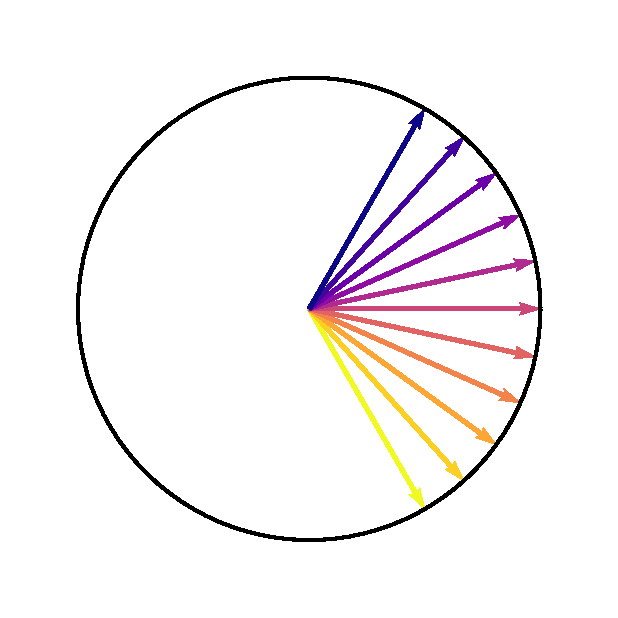
\includegraphics[width=1\textwidth]{Theory/SE/se_spins_t_te_inverted.eps}
		\caption{After 180$\degree$ pulse}
		\label{fig:theory_se_spins_t_te_by_2_inverted}
	\end{subfigure}
	\begin{subfigure}[c]{0.24\textwidth}
		\centering
		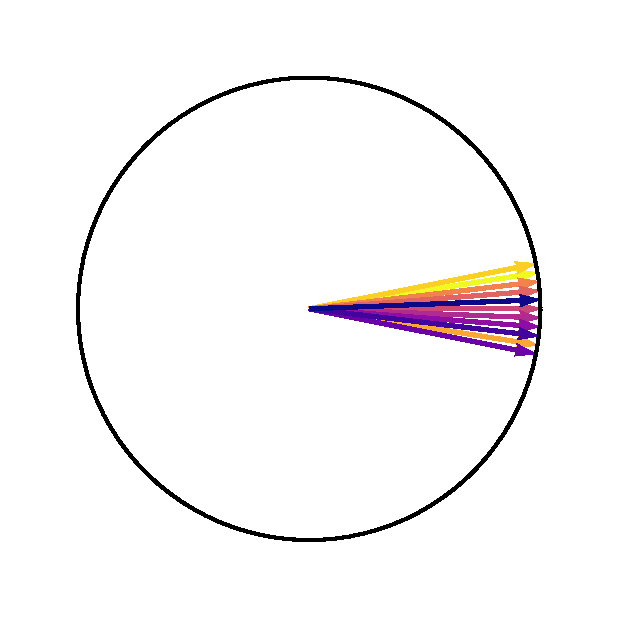
\includegraphics[width=1\textwidth]{Theory/SE/se_spins_t_2te.eps}
		\caption{$t$ = 2TE}
		\label{fig:theory_se_spins_t_te}
	\end{subfigure}
	\caption{Spins evolving in a spin echo sequence showing the de-phasing, (\subref{fig:theory_se_spins_t_te_by_2}), refocusing pulse, (\subref{fig:theory_se_spins_t_te_by_2_inverted}), and subsequent refocusing, (\subref{fig:theory_se_spins_t_te}).}
	\label{fig:theory_se_spins}
\end{figure}

By repeating this sequence over a range of echo times the \ttwo curve can be sampled and fit to \eqref{eq:theory_bloch_transverse_mxy} to estimate \ttwo and $M_{xy\; 0}$. The \ac{SE} sequence is the most basic form of \ttwo mapping, more methods are explored and compared in Chapter \ref{chap:t2_mapping} of this thesis.

\subsubsection{Gradient Echoes}
\label{subsubsec:theory_ge}
Echoes can be generated via another mechanism, the \ac{GE}. In addition to the homogenous $B_0$ field and \ac{RF} fields encountered thus far, \ac{MRI} scanners can produce additional fields known as gradients. These switchable fields can induce linearly varying spatially dependent magnetic fields to perturb $B_0$. They are used for image formation, explained in Section \ref{sec:theory_forming_an_image} but can also be used to form an echo. The \ac{GE} pulse sequence uses a single 90\degree{ }\ac{RF} excitation pulse to tip the net magnetisation vector into the transverse plane. A gradient is then applied to the sample causing areas of higher field to de-phase quickly whereas areas with a relatively lower field will de-phase slower. At time \ac{TE}/2 the polarity of the gradient is reversed thus causing the spins to refocus and an echo to be formed at time \ac{TE}. An overview of the sequence is shown in Figure \ref{fig:theory_ge_signal}. 

\begin{figure}[H]
	\centering
	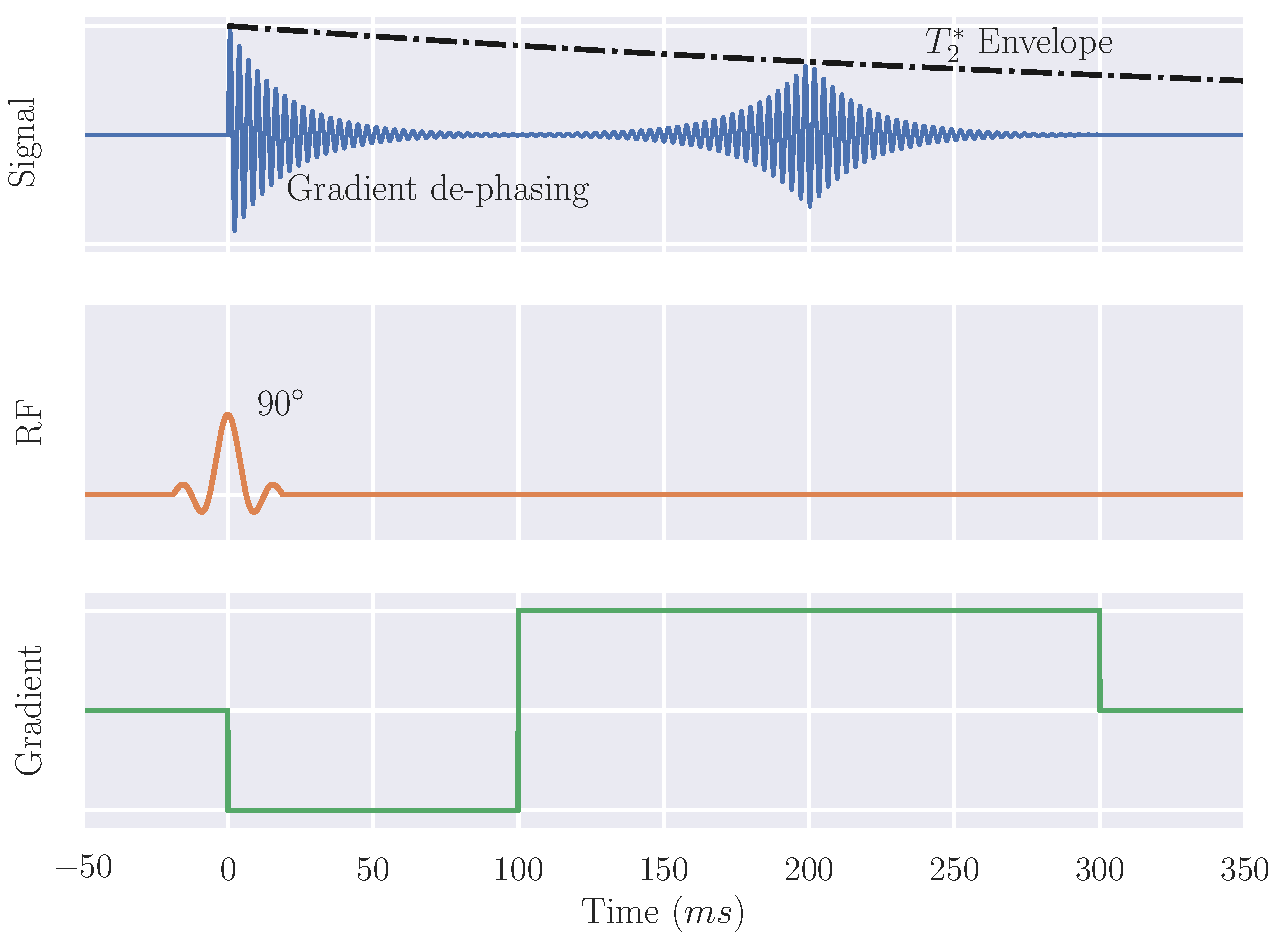
\includegraphics[width=0.8\textwidth]{Theory/GE/ge_signal.eps}
	\caption{A schematic of a basic \acf{GE} sequence with \ac{TE} 200 ms.}
	\label{fig:theory_ge_signal}	
\end{figure}

In reality, the gradients cannot switch polarity instantaneously due to the inductance of the gradient coils and characteristics of the amplifiers used to generate the gradients. This phenomenon leads to the gradient waveform being trapezoidal, however, to aid clarity in schematics within this chapter, an idealised gradient waveform has been shown. This characteristic of a gradient is known as the slew rate and is defined as the peak gradient amplitude upon the rise time, Figure \ref{fig:theory_slew}, and for modern \ac{MRI} scanners is of the order of 200 T/m/s.

\begin{figure}[H]
	\centering
	\includegraphics[width=0.6\textwidth]{Theory/GE/slew.pdf}
	\caption{A gradient waveform with typical peak gradient amplitude, rise time and slew rate.}
	\label{fig:theory_slew}	
\end{figure}

\subsection{Dipole-Dipole Interactions}
\label{subsec:theory_dipole_dipole_interactions}
As outlined in \ref{subsec:theory_t1} and \ref{subsec:theory_t2}, dipole-dipole interactions are a primary contributing factor to \tone and \ttwo times. The factors that dictate the strength of these interactions are the types of spin involved, the distance between them, the angle between them and their motion. The strength of the interaction depends on the gyromagnetic ratio of the spins involved. The magnitude of an electrons gyromagnetic ratio is much greater than that of a proton (-28025 MHzT$^{-1}$ and 43 MHzT$^{-1}$ respectively \cite{mohr_codata_2016}) and as such proton-electron interactions are much stronger than proton-proton interactions. The strength of the interaction is inversely proportional to the sixth power of distance (seen in Equations \eqref{eq:theory_SB_t1} and \eqref{eq:theory_SB_t2}) and thus means that dipole-dipole interactions are only effective over a very short range. As such, the majority of interactions are intramolecular rather than intermolecular.

The $z$ component of a magnetic field produced by a dipole, $\bm{\mu}$, is given by Equation \ref{eq:theory_dipole_z},
\begin{equation}
	B_{\mu z} \propto \frac{\mu}{r^3}\left( 3\cos^2\theta -1\right) 
	\label{eq:theory_dipole_z}
\end{equation}
producing the field shown in Figure \ref{fig:theory_magic_angle}. Here it can be seen that at a certain angle, the magnetic field is zero, this occurs when $\left( 3\cos^2\theta -1\right) = 0$ and equates to an angle of approximately $54.7\degree$. This angle is known as the magic angle. If the dipoles are orientated at approximately the magic angle to the $B_0$ field, their \ttwo will be increased.


\begin{figure}[H]
	\centering
	\includegraphics[width=0.6\textwidth]{Theory/Correlation_Time/magic_angle.pdf}
	\caption{The $z$ component of the magnetic field produced by dipole, $\mu$.}
	\label{fig:theory_magic_angle}	
\end{figure}

Molecules can move in three different ways, translation, vibration and rotation. Translation has little effect on \ac{NMR} signals as it is usually omnidirectional. Vibrational oscillations are at a much higher frequency than \ac{NMR} phenomenon and as such do not affect the \ac{MRI} signal. Rotations can be at similar frequencies to \ac{MRI} and as such, influence \tone and \ttwo due to dipole-dipole interactions.

Each molecule in a sample will have a characteristic correlation time, $\tau_c$, the time it takes the molecule to rotate by one radian. The correlation time is effected by how tightly bound the molecules are and their mass, light freely bound molecules like water in liquid form will have a short correlation time while heavy tightly bound molecules such as those found in bone, will have a longer correlation time. If a molecule is tumbling at a rate similar to the Larmor frequency, it will cause energy transfer to be more efficient, thus reducing \tone. As the tumbling rate slows, the properties of the dipole become more similar to those of a static field, this means that nearby dipoles will experience magnetic fields perpetuated about $B_0$ and as such \ttwo will decrease.

The mathematical framework of this phenomenon is given by the Solomon-Bloembergen equations \cite{solomon_relaxation_1955} (Equations \eqref{eq:theory_SB_t1} and \eqref{eq:theory_SB_t2}). These equations predict \tone and \ttwo dependence on correlation time, Figure \ref{fig:theory_relaxation_correlation}, where it can be observed that \tone is lowest when the frequency of the molecular tumbling is similar to the Larmor frequency (labelled as $\tau_0$ where $\tau_0=\sfrac{1}{\omega_0}$) and that \ttwo decreases as correlation time increases. Tissues with a range of tumbling rates are highlighted in Figure \ref{fig:theory_relaxation_correlation}; the molecules in \ac{CSF} are weakly bound as they are in the liquid phase, whereas solid tissues such as bone are tightly bound. Renal tissue is expected to have a similar tumbling rate to muscle and cysts a similar tumbling rate to \ac{CSF}.

\begin{eqnarray}
	\frac{1}{T_1}&=& \frac{6}{20}\frac{\hbar^2\gamma^4}{r^6}\left[ \frac{\tau_c}{1 + \omega^2\tau_c^2} + \frac{4\tau_c}{1 + 4\omega^2\tau_c^2}\right]
	\label{eq:theory_SB_t1}\\
	\frac{1}{T_2}&=& \frac{3}{20}\frac{\hbar^2\gamma^4}{r^6}\left[ 3\tau_c +  \frac{5\tau_c}{1 + \omega^2\tau_c^2} + \frac{2\tau_c}{1 + 4\omega^2\tau_c^2}\right]
	\label{eq:theory_SB_t2}
\end{eqnarray}
\begin{figure}[H]
	\centering
	\includegraphics[width=0.7\textwidth]{Theory/Correlation_Time/relaxation_correlation.pdf}
	\caption{\tone and \ttwo dependence on molecular correlation time as predicted by the Solomon-Bloembergen equations. Tissues with a range of correlation times are highlighted.}
	\label{fig:theory_relaxation_correlation}	
\end{figure}

%\begin{figure}[H]
%	\centering
%	\includegraphics[width=0.7\textwidth]{Theory/Correlation_Time/relaxation_b0.pdf}
%	\caption{}
%	\label{fig:theory_relaxation_b0}	
%\end{figure}

\subsection{Diffusion Weighted Imaging}
\label{subsec:theory_diffusion}
Spins have been considered stationary until Section \ref{subsec:theory_dipole_dipole_interactions}. In biological tissues, they will undergo Brownian motion leading to diffusion. The signal from a sample can be made sensitive to the degree of diffusion taking place by using diffusion gradients applied between the excitation and echo. 

Figure \ref{fig:theory_diffusion_psd} shows a \ac{DWI} pulse sequence and the phase evolution of two spins, one stationary and the other diffusing along the direction in which the diffusion gradient is applied. The stationary spin accrues a positive phase shift relative to $\omega_0$ while the first diffusion gradient pulse is applied. The 180$\degree$ \ac{RF} pulse then flips the spin system so the positive phase shift reverses to a negative phase shift of equal magnitude. The spin then evolves under the same field strength in the second diffusion gradient pulse and as such, the diffusion pulses result in no net phase shift. In contrast, for the diffusing spin,the strength of the magnetic field experienced is dependent on time, in this example, increasing in strength as time passes. This means that the rate at which phase shifts are accrued increases over time and therefore the refocussing effects of the second diffusion pulse are reduced. This sensitivity of the diffusion sequence to water motion is dependent on the strength of the diffusion gradients, the time the diffusion gradients are applied for and the time between the two diffusion pulses. This is termed the diffusion weighting factor, b, and for a monopolar Stejskal-Tanner sequence is given by \eqref{eq:theory_stejskal_tanner} where b has units of s/mm$^2$, $G$ is the amplitude of the gradient, $\delta$ is the duration of the gradient and $\Delta$ is the time interval \cite{stejskal_spin_1965}. To increase the b-value, either the gradient amplitude or duration of time interval can be increased, however it is often preferable to adjust b-values purely by altering the gradient amplitude to keep the diffusion time constant.

\begin{equation}
	b=\gamma^2 G^2 \delta^2 \left( \Delta - \sfrac{\delta}{3}\right)
	\label{eq:theory_stejskal_tanner}
\end{equation}

\begin{figure}[H]
	\centering
	\includegraphics[width=0.8\textwidth]{Theory/Diffusion/diffusion_psd.pdf}
	\caption{Phase evolution of two spins under the influence of monopolar diffusion encoding gradients.}
	\label{fig:theory_diffusion_psd}	
\end{figure}

The interplay between diffusion gradients and measured signal can be mathematically modelled by Equation \eqref{eq:theory_adc},
\begin{equation}
	S\left( b \right) = S_0 \cdot e^{-b \cdot ADC},
	\label{eq:theory_adc}
\end{equation}
where b is the b-value, and \acs{ADC} is the \acl{ADC} of the tissue and reflects the degree with which spins can diffuse through a tissue, given in mm$^2$/sec. By repeating the acquisition with different b-values, the signal from each voxel at each b-value can be used to estimate \ac{ADC} (and $S_0$) by fitting the data to Equation \eqref{eq:theory_adc}.

For large b-values, typically greater than 250 s/mm$^2$, diffusion is the primary contributing factor to signal attenuation. For b-values less than 250 s/mm$^2$ an additional mechanism in the form of perfusion, micro-circulation of blood in capillaries, leads to additional signal attenuation. This additional factor can be modelled by the \ac{IVIM} model, \eqref{eq:theory_ivim}, where $f$ is the perfusion fraction, the proportion of a voxels volume occupied by capillaries, $D$ is the tissues diffusion coefficient and $D^*$ is the pseudodiffusion coefficient, reflecting the additional de-phasing due to perfusion within capillaries in a voxel \cite{le_bihan_mr_1986,le_bihan_separation_1988}.

\begin{equation}
	S\left( b \right) = S_0 \left[ f \cdot e^{-b\left(D + D^*\right)} + \left( 1 - f\right) \cdot e^{-b \cdot D}\right]
	\label{eq:theory_ivim}
\end{equation}

By acquiring data at a range of b-values, ensuring that low b-values are well sampled, a voxel by voxel fit can be performed to estimate $f$, $D$ and $D^*$.

Not all diffusion is isotropic (occurs to the the same degree in all directions), often the motion of the spins is restricted e.g. within tissue fibres. The amount of restriction is known as the \ac{FA} where 0 represents isotropic diffusion e.g. a large vial of water, and 1 represents diffusion being constrained to a single dimension. By applying the diffusion gradients in different directions (and strengths) the preferred direction of diffusion and fractional anisotropy can be calculated. These techniques are used in Chapter \ref{chap:ex} to study \ac{DTI} in ex-vivo tissue samples.

\subsection{Optimisation of Tissue Contrast}
\label{subsec:theory_optimising_contrast}
Quantitative mapping of \tone, \ttwo and \ttwostar can often be a slow process due to the number of acquisitions required at different time points to sample relaxation curves. Often it is more desirable to acquire a volume at a single inversion/echo time with the intensity difference between tissues of interest maximised. Although the voxel intensities do not directly represent any quantitative underlying physical properties of the tissue, the contrast between tissues is sufficient for diagnosis or further analysis. For example, in Chapter \ref{chap:ML} optimised contrast between organs is used for segmentation of the kidneys.

\begin{figure}[H]
	\centering
	\begin{subfigure}[c]{1\textwidth}
		\centering
		\includegraphics[width=0.8\textwidth]{Theory/Tissue_Contrast/tissue_contrast_t1.eps}
		\caption{}
		\label{fig:theorgy_tissue_contrast_t1}
	\end{subfigure}
	\vskip\baselineskip
	\begin{subfigure}[c]{1\textwidth}
		\centering
		\includegraphics[width=0.8\textwidth]{Theory/Tissue_Contrast/tissue_contrast_t2.eps}
		\caption{}
		\label{fig:theorgy_tissue_contrast_t2}
	\end{subfigure}
	\caption{(\subref{fig:theorgy_tissue_contrast_t1}) The signal generated from renal cortical and medullary tissues \cite{cox_multiparametric_2017} following an inversion recovery and difference between signals. This shows that the contrast between the two tissues is optimal if the \acf{TI} is 1500 ms. (\subref{fig:theorgy_tissue_contrast_t2}) The signal generated from the kidneys, liver and spleen following a spin echo sequence and the difference between the signals.}
	\label{fig:theorgy_tissue_contrast}
\end{figure}

\section{Forming an Image}
\label{sec:theory_forming_an_image}
\subsection{Signal Localisation}
So far, \ac{NMR} has been applied to measure signals from the entire sample, gaining no information about the spatial variation within it. \ac{MRI} applies the techniques of \ac{NMR} to spatially resolve the location of the signal.

The key concepts of \ac{MRI} were developed by multiple groups in the 1970s. Lauterbur used magnetic field gradients and a back-projection reconstruction technique to generate 2D images in 1973 \cite{lauterbur_image_1973}. Simultaneously Mansfield was working on ``\ac{NMR} diffraction'' introducing the mathematical framework of reciprocal $k$-space \cite{mansfield_nmr_1973} and later slice selective excitation \cite{garroway_image_1974}. The final key insight was provided by Ernst who published the first Fourier imaging method \cite{kumar_nmr_1975}, this used non-selective excitations and linear gradients to generate 2D Fourier encoded images. These techniques are still the basis of \ac{MRI} today.

The concepts of signal localisation will be introduced through the example of an axial acquisition, Figure \ref{fig:theory_axial_planning}. Throughout this chapter, the brain is used for examples of image formation as this anatomy highlights some of the concepts discussed more clearly. A typical series of equivalent renal scans is shown in Figure \ref{fig:theory_renal_localisers}.
\begin{figure}[H]
	\centering
	\includegraphics[width=0.8\textwidth]{Theory/Signal_Localisation/signal_localisation_planning.eps}
	\caption{Planning used in the signal localisation example.}
	\label{fig:theory_axial_planning}	
\end{figure}

\begin{figure}[H]
	\centering
	\includegraphics[width=0.8\textwidth]{Theory/Signal_Localisation/renal_localisers.eps}
	\caption{Typical localisers used to plan further renal scans.}
	\label{fig:theory_renal_localisers}	
\end{figure}
\subsubsection{Gradient Fields}
Signal localisation makes use of gradient fields. These produce small linear perturbations in $B_0$ and are applied in a combination of the $x$, $y$ and $z$ direction to enable arbitrary gradient directions and result in $B_0$ varying with spatial position, $\mathbf{r}$,
\begin{equation}
B_z\left( r\right) =\left( B_0 + \mathbf{G \cdot r}\right) \hat{k}.
\end{equation}
As such, the resonant frequency of the spins can also be described as a function of position and, because the gradients are not static, also in time;
\begin{equation}
\omega\left( x, y, z, t \right) = \gamma \left( B_0 + G_x(t)x + G_y(t)y + G_z(t)z \right) 
\label{eq:theory_localisation_gradients}
\end{equation}

\subsubsection{Slice Selection}
The initial step in localisation is to measure the signal from a single, spatially defined, slice. If a gradient is applied along the $z$ direction, $G_z$, the magnetic field experienced by the spins at position $z$ will be
\begin{equation}
B\left( z\right)  = B_0 + G_zz.
\end{equation}
As such, from the simplification of \eqref{eq:theory_localisation_gradients}, the Larmor frequency becomes
\begin{equation}
\omega\left( z\right)  = \gamma\left( B_0 + G_zz\right).
\end{equation}
If a frequency selective \ac{RF} pulse is applied to the sample, it will only excite spins within the corresponding bandwidth and thus only a slice of desired thickness. This slice-selective thickness, $\Delta z$, can be changed by either adjusting the amplitude of $G_z$ or the bandwidth of the excitation \ac{RF} pulse, $\Delta \omega$.
\begin{equation}
\Delta z = \frac{\Delta \omega}{\gamma G_z}
\end{equation}

The excitation profile achieved by a slice selective pulse can be approximated by a Fourier transform. Generally, a rectangular slice profile is wanted and as such, the \ac{RF} pulse takes the form of a sinc function. To achieve a perfect rectangular pulse, the sinc would have to be infinite in length. Given the lack of infinite time available during an \ac{MRI} examination, a truncated sinc pulse is used, generally including three or five lobes and a Gaussian filter.

The gradient applied will result in de-phasing of the spins as in a \ac{GE} sequence, therefore a gradient of the opposite polarity and half the magnitude is applied after the \ac{RF} pulse to re-phase the spins, Figure \ref{fig:theory_slice_select_rephasing}.

\begin{figure}[H]
	\centering
	\begin{subfigure}[c]{0.47\textwidth}
		\centering
		\includegraphics[width=1\textwidth]{Theory/Slice_Select/slice_select_rephasing.eps}
		\caption{}
		\label{fig:theory_slice_select_rephasing}
	\end{subfigure}
	\hfill
	\begin{subfigure}[c]{0.47\textwidth}
		\centering
		\includegraphics[width=1\textwidth]{Theory/Slice_Select/slice_select.eps}
		\caption{}
		\label{fig:theory_slice_select_profile}
	\end{subfigure}
	\caption{(\subref{fig:theory_slice_select_rephasing}) A truncated sinc pulse of bandwidth $\Delta \omega$ is applied at the same time as a slice selective gradient, this is followed by the negative re-phasing gradient lobe. Note that the area under the re-phasing gradient is half that of the slice selective gradient. (\subref{fig:theory_slice_select_profile}) Example slices of thickness $\Delta z$ being excited by \ac{RF} pulses of bandwidth $\Delta \omega$, showing that excitation pulses with larger bandwidth result in thicker slice profiles.}
	\label{fig:theory_slice_select}
\end{figure}
\subsubsection{Phase Encoding}
So far, the signal has been localised from a full 3D volume to a defined 2D volumetric slice. To localise the signal in the next dimension, phase encoding is used. This technique uses a gradient in the $y$ direction applied for time $T$. For the duration of $G_y$ the spins precess with a frequency according to their position in the $y$ direction
\begin{equation}
\omega \left( y\right) = \gamma\left( B_0 + G_yy\right),
\end{equation}
and as such accrue a phase shift, $\phi \left( y \right)$, relative to the situation if no gradient was applied. This is given by 
\begin{equation}
\phi\left( y\right)  = \gamma y \int_{0}^{T} G_y\left( t\right) dt.
\end{equation}
Acquisitions must be repeated with different amplitudes/durations of $G_y$ to fully sample the $y$ direction.

Phase aliasing occurs because the whole sample produces signal, whether it is in the \ac{FOV} or not. As there is a finite range of phase values ($0$ to $2\pi$) tissue outside the \ac{FOV} can have the same value as tissue within the \ac{FOV}, this results in the two signals becoming indistinguishable and therefore combined in a process known as wrapping. This artefact is illustrated in Figure \ref{fig:theory_wrapping_spins} using the brain because its simple oval shape lends itself to a clearer diagram. This artefact is just as, if not more, prevalent in the body where there is a much larger variance in subject size and thus, in the interest of consistent protocols, larger \acp{FOV} are acquired, slowing the acquisition.
\begin{figure}[H]
	\centering
	\includegraphics[width=0.4\textwidth]{Theory/kspace/wrapping_spins.pdf}
	\caption{Spins outside the \ac{FOV} have the same phase value as those within the \ac{FOV} and thus wrapping occurs.}
	\label{fig:theory_wrapping_spins}	
\end{figure}

\subsubsection{Frequency Encoding}
Finally, the signal needs to be localised in the $x$ direction. This is achieved using frequency encoding. Here the gradient, $G_x$ is applied during the acquisition component of the sequence i.e. when the signal is being sampled. As the gradient is applied during readout, those spins in the centre of the gradient (at field $B_0$) will precess at the Larmor frequency while those in a stronger or weaker field will precess faster or slower respectively. By sampling the signal generated and applying a Fourier transform to separate components of the signal at each frequency, the signal is spatially resolved in all three dimensions. An overview of a basic signal localisation scheme is shown in Figure \ref{fig:theory_signal_loc}.
\begin{figure}[H]
	\centering
	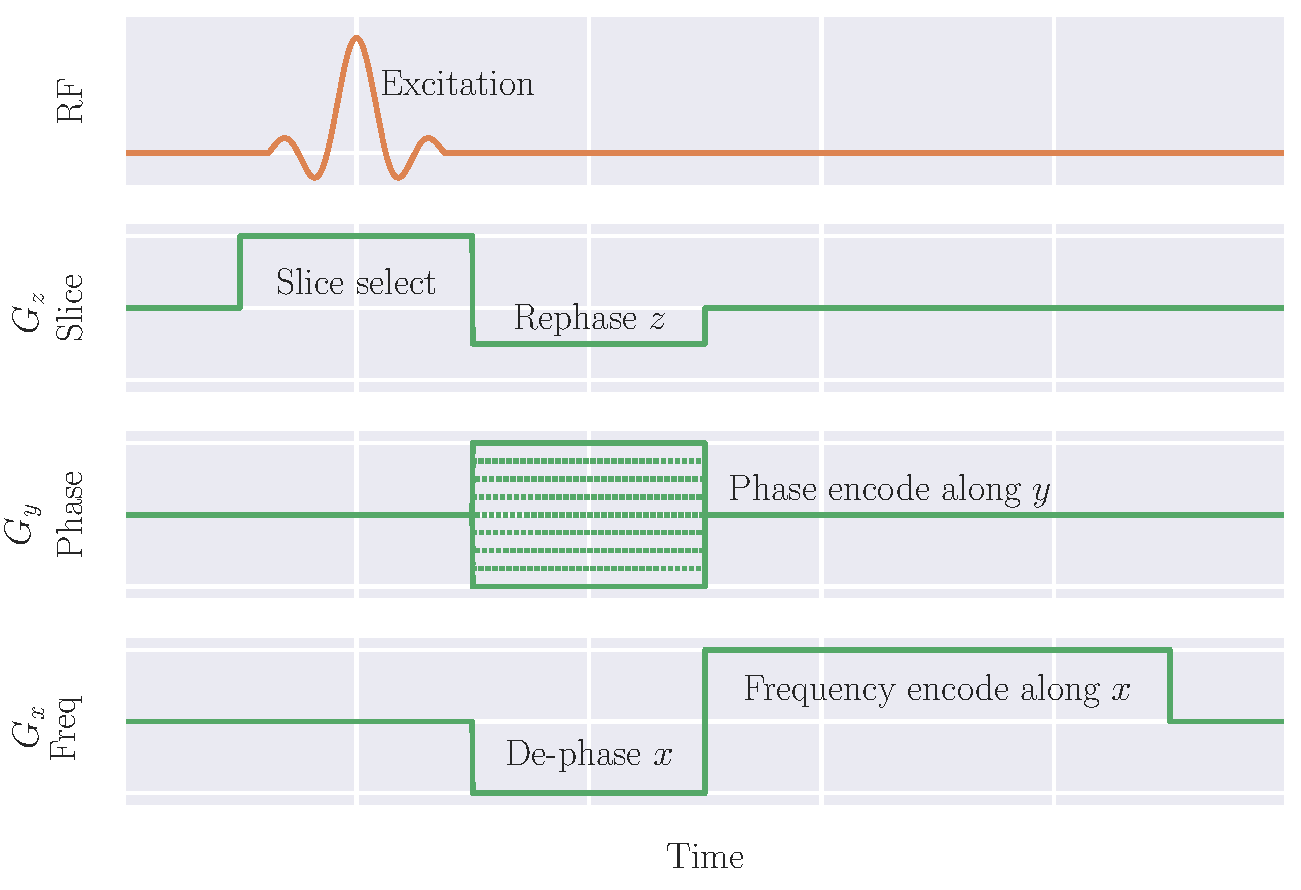
\includegraphics[width=0.8\textwidth]{Theory/Signal_Localisation/signal_localisation_psd.eps}
	\caption{A basic spacial localisation pulse sequence showing how gradients applied along the $z$, $y$ and $x$ directions can be used to localise the signal in the corresponding dimensions. The repetitions with different phase encoding gradient amplitudes are represented by the dotted lines in $G_y$.}
	\label{fig:theory_signal_loc}	
\end{figure}

\subsubsection{$k$-space}
$k$-space, sometimes known as Fourier space, is a useful concept for interpreting \ac{MRI} pulse sequences and represents the spatial frequencies of the image. Immediately after an excitation pulse and rewind gradient, the signal being sampled is at the origin of $k$-space, corresponding to low spatial frequencies, or the low resolution aspects of the image e.g. which voxels are inside or outside the body. As gradients are applied to the sample, sampling moves out from the centre of $k$-space to higher spatial frequencies corresponding to finer detail within the image. For a 2D acquisition, as above, the location in $k$-space is defined by \eqref{eq:theory_k_space_x} and \eqref{eq:theory_k_space_y} where $G_x$ and $G_y$ are the gradients in the frequency encode and phase encode directions respectively and $t_x$ and $t_y$ are the duration the gradient is applied for.
\begin{eqnarray}
k_x &=& \gamma G_x t_x
\label{eq:theory_k_space_x} \\
k_y &=& \gamma G_y t_y
\label{eq:theory_k_space_y}
\end{eqnarray}

When recording \ac{MRI} data, the continuous signal must be discretised. The higher the sampling frequency i.e. the closer together in $k$-space the samples are, $\Delta k$, the wider the \ac{FOV} and the further out from the origin of $k$-space is samples, the higher resolution the image will be. Examples of $k$-space sampling patterns and their corresponding image are shown in Figure \ref{fig:theory_kspace}.

\begin{figure}[h!]
	\centering
	\begin{subfigure}[c]{0.8\textwidth}
		\centering
		\includegraphics[width=1\textwidth]{Theory/kspace/kspace_full_sample.eps}
		\caption{}
		\label{fig:theory_kspace_full}
	\end{subfigure}
	\vskip\baselineskip
	\begin{subfigure}[c]{0.8\textwidth}
		\centering
		\includegraphics[width=1\textwidth]{Theory/kspace/kspace_centre.eps}
		\caption{}
		\label{fig:theory_kspace_centre}
	\end{subfigure}
	\vskip\baselineskip
	\begin{subfigure}[c]{0.8\textwidth}
		\centering
		\includegraphics[width=1\textwidth]{Theory/kspace/kspace_wrap.eps}
		\caption{}
		\label{fig:theory_kspace_wrap}
	\end{subfigure}
	\caption{(\subref{fig:theory_kspace_full}) Fully samples $k$-space and the corresponding image. (\subref{fig:theory_kspace_centre}) Centre sampling of $k$-space produces a lower resolution image. (\subref{fig:theory_kspace_wrap}) Sampling with a larger $\Delta k$ resulting in a decreased \ac{FOV} and aliasing.}
	\label{fig:theory_kspace}
\end{figure}

\subsubsection{From $k$-space to Image Space}

The raw data sampled in $k$-space can be reconstructed to an image via a Fourier transform. When the quadrature data undergoes a 2D Fourier transform, it produces a complex image composed of a real and imaginary part. These constituent parts of the image can be converted into magnitude and phase images with the magnitude representing the spin density.

\subsubsection{Coordinate Systems}
The above example was chosen so that only one gradient is used at once however if the planning of the acquisition is more complicated, the nomencleture can become more confusing, as such, for clarity multiple coordinate systems are often used.
\paragraph{Scanner Space:}
This coordinate system has its origin at isocentre of the scanner and is defined in terms of $x$, $y$ and $z$.
\paragraph{Imaging Space:}
The coordinates of this system are defined by the directions used in signal localisation, $M$ for the frequency encode direction (also called magnitude), $P$ for the phase encode direction and $S$ for the slice select direction.
\paragraph{Anatomical Space:}
Defined in terms of the subjects orientation in the scanner, this coordinate system has the axis, Right-Left (R-L), Anterior-Posterior (A-P) and Superior-Inferior (S-I).

\subsection{Image Acquisition Acceleration}
One of the recurring limiting factors in \ac{MRI} is the acquisition time. For neuroimaging applications, the relatively slow acquisition of \ac{MRI} limits subject throughput or the number of different measures that can be performed. In abdominal imaging, acquisition times can be even more of a hindrance given many scans are performed while the subject is holding their breath on expiration as typically used in this thesis. As such, image acquisition acceleration techniques have been developed. These techniques sacrifice a small amount of \ac{SNR} for a decrease in acquisition time.

\subsubsection{Partial Fourier}
\label{subsec:theory_partial_fourier}
Fully sampled $k$-space contains inherent redundancy as it contains its own complex conjugate; the real components of the signal are symmetric while the imaginary components are anti-symmetric. This means that theoretically no contrast information is lost if a reduced area of $k$-space is sampled e.g. only 66\% of $k$-space is sampled. However, this technique does impact phase information and so should not be used in acquisitions where downstream processing requires accurate phase. Known as partial Fourier or halfscan, this technique results in a decreased \ac{SNR} and can introduces image artefacts as the partial Fourier factor approaches 50\%, however, the acquisition time reduces by approximately the percentage of $k$-space sampled e.g. an acquisition that would take three minutes fully sampled will take two minutes if a partial Fourier factor of 66\% is used. An example of reconstructions of 100\%, 75\% and 51\% of $k$-space are shown in Figure \ref{fig:theory_partial_fourier}

\begin{figure}[h!]
	\centering
	\begin{subfigure}[c]{0.30\textwidth}
		\centering
		\includegraphics[width=1\textwidth]{Theory/partial_fourier/kspace_full.eps}
		\caption{}
		\label{fig:theory_partial_fourier_full_k}
	\end{subfigure}
	\hfill
	\begin{subfigure}[c]{0.30\textwidth}
		\centering
		\includegraphics[width=1\textwidth]{Theory/partial_fourier/kspace_75.eps}
		\caption{}
		\label{fig:theory_partial_fourier_75_k}
	\end{subfigure}
	\hfill
	\begin{subfigure}[c]{0.30\textwidth}
		\centering
		\includegraphics[width=1\textwidth]{Theory/partial_fourier/kspace_51.eps}
		\caption{}
		\label{fig:theory_partial_fourier_51_k}
	\end{subfigure}
\vskip\baselineskip
	\begin{subfigure}[c]{0.30\textwidth}
		\centering
		\includegraphics[width=1\textwidth]{Theory/partial_fourier/image_full.eps}
		\caption{}
		\label{fig:theory_partial_fourier_full_image}
	\end{subfigure}
	\hfill
	\begin{subfigure}[c]{0.30\textwidth}
		\centering
		\includegraphics[width=1\textwidth]{Theory/partial_fourier/image_75.eps}
		\caption{}
		\label{fig:theory_partial_fourier_75_image}
	\end{subfigure}
	\hfill
	\begin{subfigure}[c]{0.30\textwidth}
		\centering
		\includegraphics[width=1\textwidth]{Theory/partial_fourier/image_51.eps}
		\caption{}
		\label{fig:theory_partial_fourier_51_image}
	\end{subfigure}
	\caption{Full, (\subref{fig:theory_partial_fourier_full_k}), 75\%, (\subref{fig:theory_partial_fourier_75_k}), and 51\%, (\subref{fig:theory_partial_fourier_51_k}), $k$-space sampling and their corresponding reconstructions in image space, (\subref{fig:theory_partial_fourier_full_image}), (\subref{fig:theory_partial_fourier_75_image}) and (\subref{fig:theory_partial_fourier_51_image}) respectively.}
	\label{fig:theory_partial_fourier}
\end{figure}

\subsubsection{\ac*{SENSE}}
Most modern scanners use different coils for \ac{RF} transmission, and signal reception. The transmission coil is usually built into the bore of the magnet while the receive coil is placed as close to the source of the signal as possible. These receive coils are usually composed of multiple smaller coils to make an array, each with its own signal sampling hardware. This means that it is possible to record signal from multiple coils simultaneously with different coils supplying data for each line of $k$-space e.g if the array has two coils, one coil will record the odd lines of $k$-space and the other, the even lines, thus resulting in an increase in acquisition speed \cite{pruessmann_sense_1999}. This parallel sampling technique reduces the lines of $k$-space sampled per coil and results in wrapping as seen in Figure \ref{fig:theory_kspace_wrap}, albeit only in the phase direction. To combat this, the spatial sensitivity profile of each element within the array i.e. the area it can measure signal from, is measured. Using this prior knowledge of signal locations, each coil elements data can be unwrapped before the data from all elements is combined into a single volume.

The \ac{SENSE} factor is the degree to which $k$-space is under-sampled and is limited to the number of elements in the receive array. Applying higher \ac{SENSE} factors increases acquisition speeds, however, reduces \ac{SNR}. This is the method implemented on Philips scanners as used in this thesis, different vendors have slightly different methodologies to accelerate imaging by utilising the limited range of elements within an \ac{RF} coil array.

\subsection{Image Acquisition Schemes}

Many different acquisition schemes have been developed for sampling $k$-space. Outlined below are some of the key sequences that form the basis of \ac{MRI} and that are employed in this thesis.

\subsubsection{Spin Warp Imaging}

The simplest uniformly sampled $k$-space trajectory is spin warp imaging. This technique is based on the \ac{GE} scheme and samples one line of $k$-space per excitation, or shot, a schematic is shown in Figure \ref{fig:theory_spin_warp}. Each shot applies a different phase encode gradient to move a different amount in the $k_y$ direction. The signal is then sampled while a gradient is applied in the frequency direction, also known as the readout gradient. The acquisition time for this sequence is very long because it only collects one line of $k$-space per shot and as such this technique is sensitive to subject motion.

\begin{figure}[H]
	\centering
	\includegraphics[width=1\textwidth]{Theory/spin_warp/spin_warp.pdf}
	\caption{A schematic of the spin warp image sequence. The \ac*{PSD} shows the different phase encoding gradients, $G_y$, in colours from yellow to purple and the readout gradient, $G_x$, in red. These colours correlate with the colours in the $k$-space trajectory. The signal recorded is highlighted in red.}
	\label{fig:theory_spin_warp}	
\end{figure}

\subsubsection{\ac*{TSE}}
\label{subsubsec:theory_tse}
The \ac{TSE} sequence, also known as \ac{FSE} or \ac{RARE}, is an expansion on the conventional \ac{SE} sequence applying evenly spaced $180\degree${ }\ac{RF} refocusing pulses to generate multiple echoes from a single excitation, these echoes are used to record multiple lines of $k$-space. The number of echoes is known as the \ac{ETL}, or `turbo factor' and is the factor by which the scan time is reduced compared to a conventional spin echo sequence, and this is anywhere between 2 and 30 per \ac{TR}; the time between echoes is known as the echo spacing and is typically of 15 - 25 ms.

Each line of $k$-space is acquired at a different time after excitation, as such the lines will have different \ttwo weightings, it is therefore important to ensure the centre of $k$-space is acquired at the desired \ac{TE} as this echo will dominate the image contrast. The time between excitation and the centre of $k$-space is known as the \ac{eTE}.

The decrease in acquisition time comes at the expense of \ac{RF} exposure, the large number of $180\degree{ }$ pulses leads to more energy in the form of heat being deposited in the tissue being imaged, this is known as \ac{SAR}. \ac{SAR} limits are imposed when scanning to avoid damaging any tissue and as such \ac{TSE} with its high \ac{RF} power can easily exceed these limits. Modern \ac{TSE} sequences can reduce the angle of the refocusing pulse, however this can come at the expense of quantitative accuracy. This sequence is discussed further in Chapter \ref{chap:t2_mapping}.

\begin{figure}[H]
	\centering
	\includegraphics[width=0.8\textwidth]{Theory/TSE/tse.pdf}
%	\missingfigure{TSE Sequence}
	\caption{A schematic of the \ac{TSE} pulse sequence and $k$-space trajectory. The coloured bands on the \ac{PSD} correspond to the colours of the $k$-space trajectories. Note this diagram is not to scale.}
	\label{fig:theory_tse}	
\end{figure}

\subsubsection{\ac*{HASTE}}
The \ac{HASTE} sequence uses a combination of the techniques above and can be seen as an extension of the \ac{TSE} sequence. A single excitation is followed by a very long echo train with short echo spacing. This allows a large proportion of $k$-space to be sampled within a single \ac{TR} and thus a whole slice is acquired. To minimise the number of lines of $k$-space acquired and thus the \ac{ETL}, partial Fourier techniques as outlined in Section \ref{subsec:theory_partial_fourier} can be utilised. The relatively long \ac{TE} required for a \ac{HASTE} sequence means images are normally \ttwo weighted. An example \ac{PSD} and $k$-space trajectory for the \ac{HASTE} sequence is shown in Figure \ref{fig:theory_haste_psd}.

\begin{figure}[H]
	\centering
	\includegraphics[width=0.8\textwidth]{Theory/HASTE/haste.pdf}
	\caption{A schematic of the \ac{HASTE} pulse sequence and $k$-space trajectory.}
	\label{fig:theory_haste_psd}	
\end{figure}

The advantage of \ac{HASTE} is its rapid acquisition. It can be used to minimise the effects of motion when scanning uncooperative patients, fetuses or structures the subject has no control over such as the bowel. Alternatively it can be used to capture a large \ac{FOV} in a single breath hold, thus minimising the effects of inconsistent expiration level, as in Chapter \ref{chap:ML}. However the very long \ac{ETL} can cause significant blurring of the image. An example abdominal \ac{HASTE} image is shown in Figure \ref{fig:theory_haste_example}.

\begin{figure}[H]
	\centering
	\includegraphics[width=0.5\textwidth]{Theory/HASTE/haste_example.png}
	\caption{An example abdominal image acquired using the \ac{HASTE} readout scheme.}
	\label{fig:theory_haste_example}
\end{figure}

\subsubsection{\ac*{TFE}}
\ac{TFE}, also known as ultrafast gradient echo, is designed to speed up the acquisition of gradient echo images by reducing the \ac{TR} between excitations. Typical basic gradient echo sequences have relatively long \ac{TR} to allow the recovery of longitudinal magnetisation. The flip angle used in the \ac{TFE} sequence is much smaller than the examples explored so far, usually approximately 10$\degree$ thus leaving a large component of the magnetisation in the longitudinal direction while tipping enough magnetisation into the transverse plane to record a signal at an acceptable \ac{SNR}. Between each excitation, the transverse magnetisation is spoiled to ensure the images are only \tone weighted. 

After a train of equally spaced \ac{RF} pulses of flip angle, $\alpha$, and period, \ac{TR}, the longitudinal magnetisation reaches a steady state, $S_{TFE}$, after a sufficient number of pulses. This steady state signal depends on the \tone of the tissue and the \ac{FA} and \ac{TR} of the sequence. Assuming perfect transverse magnetisation spoiling between each \ac{RF} pulse, this equilibrium signal is given by,

\begin{equation}
	S_{TFE} = M_0 \frac{\sin \left( \alpha \right) \left[ 1 - \exp \left( -\sfrac{TR}{T_1}\right) \right]}{1-\cos \left( \alpha \right) \exp \left( -\sfrac{TR}{T_1}\right)} \exp \left( - \frac{TE}{T_2^*}\right).
	\label{eq:tfe_signal}
\end{equation}

The angle that produces the maximum signal, known as the Ernst angle, $\alpha_E$, is given by,
\begin{equation}
	\alpha_E = \arccos \left[ \exp \left( -\frac{TR}{T_1}\right)\right].
	\label{eq:theory_ernst}
\end{equation}
Figure \ref{fig:theory_ernst} shows the ratio of the steady state signal to the fully recovered, 90$\degree${ } excitation signal of renal cortex (\tone of 1376 ms) for a range of flip angles and \ac{TR}. Additionally the Ernst angle is shown. 
\begin{figure}[H]
	\centering
	\includegraphics[width=0.7\textwidth]{Theory/TFE/ernst.pdf}
	\caption{The expected steady state signal of a \ac{TFE} pulse sequence and Ernst angle when imaging renal cortex.}
	\label{fig:theory_ernst}	
\end{figure}

An example \ac{TFE} pulse sequence is shown in Figure \ref{fig:theory_tfe_psd}. This schematic includes three startup echoes while the longitudinal magnetisation reaches a steady state then sixteen echoes where the signal is sampled to form an image.
\begin{figure}[H]
	\centering
	\includegraphics[width=0.8\textwidth]{Theory/TFE/tfe.pdf}
	\caption{A schematic of the \ac{TFE} pulse sequence. Startup echoes are highlighted in blue, echoes used in image acquisition are highlighted in red.}
	\label{fig:theory_tfe_psd}
\end{figure}
An image generated using a \ac{TFE} sequence is shown in Figure \ref{fig:theory_tfe_example}.
\begin{figure}[H]
	\centering
	\includegraphics[width=0.5\textwidth]{ML/T1/T1W.png}
	\caption{An example of an abdominal image acquired using the \ac{TFE} scheme. This \tone-weighted image is used to segment the renal cortex and medulla.}
	\label{fig:theory_tfe_example}	
\end{figure}

\subsubsection{\ac*{EPI}}
A much faster imaging technique is \ac{EPI} \cite{mansfield_nmr_1973}. This technique samples all lines of $k$-space in a single excitation shot with an acquisition time typically less than 100 ms. The \ac{PSD} and $k$-space trajectory for this sequence are shown in Figure \ref{fig:theory_epi}. The sequence begins with a slice selective excitation and an acquisition of the bottom line of $k$-space, however, instead of a spoiler followed by another excitation as in spin warp imaging, in \ac{EPI} a small positive phase encode gradient `blip' is applied to move up a line in $k$-space, followed by an inversion of the readout gradient polarity. This blip followed by reversed readout is repeated, zig-zagging up $k$-space until the desired $k$-space is sampled.

\begin{figure}[H]
	\centering
	\includegraphics[width=1\textwidth]{Theory/EPI/epi.pdf}
	%	\missingfigure{EPI PSD and k-space}
	\caption{A schematic of the \ac{GE}-\ac{EPI} pulse sequence and $k$-space trajectory. This diagram is not to scale.}
	\label{fig:theory_epi}	
\end{figure}

While this sequence has a very short acquisition time, it does have drawbacks. The long train of echoes makes \ac{EPI} more sensitive to inhomogeneities in the $B_0$ field caused by different tissue susceptibilities or poor shimming. Eddy currents and imperfections in gradient coils cause small differences in lines collected in the positive and negative direction, leading the a Nyquist ghost artefact. Eddy currents induced by the phase encode blips also cause geometric distortions in the image, Figure \ref{fig:theory_epi_eddy}, however, these can be corrected via post processing if an image with phase encode blips of opposite polarity is collected i.e. collect images sampling $k$-space from both bottom to top and top to bottom. This is outlined further in Chapter \ref{chap:ex}

\begin{figure}[H]
	\centering
	\begin{subfigure}[c]{0.30\textwidth}
		\centering
		\includegraphics[width=1\textwidth]{Theory/EPI/blip_l.png}
		\caption{}
		\label{fig:theory_epi_blip_l}
	\end{subfigure}
	\hfill
	\begin{subfigure}[c]{0.30\textwidth}
		\centering
		\includegraphics[width=1\textwidth]{Theory/EPI/blip_r.png}
		\caption{}
		\label{fig:theory_epi_blip_r}
	\end{subfigure}
	\hfill	
	\begin{subfigure}[c]{0.30\textwidth}
		\centering
		\includegraphics[width=1\textwidth]{Theory/EPI/blip_corrected.png}
		\caption{}
		\label{fig:theory_epi_blip_corrected}
	\end{subfigure}
	\caption{Geometric distortions in a \ac{SE}-\ac{EPI} when phase encode blips are (\subref{fig:theory_epi_blip_l}) positive, (\subref{fig:theory_epi_blip_r}) negative and (\subref{fig:theory_epi_blip_corrected}) corrected via post processing.}
	\label{fig:theory_epi_eddy}
\end{figure}

\section{Conclusion}
This chapter has introduced the basic concepts of \ac{NMR} and \ac{MRI} required for interpreting this thesis. These techniques are built upon in the experimental chapters for quantification of renal properties, both in-vivo and ex-vivo.

\newpage
\section{References}
\defbibheading{bibliography}[\refname]{}
\printbibliography